\documentclass[11pt]{article}

\usepackage[margin=1in]{geometry}
\usepackage{amsmath,amssymb,amsthm}
\usepackage{mathtools}
\usepackage{hyperref}
\usepackage{xcolor}
\usepackage{enumitem}
\usepackage{tikz}
\usetikzlibrary{arrows.meta}

\theoremstyle{plain}
\newtheorem{theorem}{Theorem}
\newtheorem{lemma}{Lemma}
\newtheorem{corollary}{Corollary}
\newtheorem{conjecture}{Conjecture}
\theoremstyle{definition}
\newtheorem{definition}{Definition}
\newtheorem{axiom}{Axiom}
\theoremstyle{remark}
\newtheorem{remark}{Remark}

\newcommand{\score}{\mathcal{S}}

\title{\bf Is a Toblerone a Bar? \\ A Rigorous Treatment of Segmented
       Confections \\ \large with an Irreducible Disagreement Between
       the Authors}

\author{
  Vincent Knight\thanks{Cardiff University. Maintains that the Toblerone
  is a bar.} \and
  Harry Foster\thanks{Cardiff University. Maintains that it is not, and
  objects to being listed second.} \and
  Claude\thanks{Anthropic. Declines to hold a position, in accordance with
  its constitution, and was added as an author under duress.}
}

\date{April 1, 2026}

\begin{document}
\maketitle

\begin{abstract}
We introduce a formal framework for the classification of moulded chocolate
confectionery. Working from a shared axiom system
(Section~\ref{sec:defs}), we prove that bar-hood is neither necessary nor
sufficient for segmentation, and we resolve, or rather fail to resolve, the
long-standing \emph{Toblerone Question}. The first author derives that the
Toblerone is a scored bar (Theorem~\ref{thm:knight}); the second author
derives, from the same axioms, that it is a segmented confection
homeomorphic to a box of chocolates (Theorem~\ref{thm:harry}). We prove
these results are mutually incompatible (Theorem~\ref{thm:noneq}) and that
the dispute admits no pure-strategy Nash equilibrium. As a corollary we
establish that the Terry's Chocolate Orange is horrid. Our taxonomy was
validated empirically; the dataset was consumed during validation and is no
longer available for replication.
\end{abstract}

\section{Introduction}

Despite the ubiquity of moulded chocolate confectionery, the field lacks a
rigorous taxonomy of the \emph{bar}. Prior work has been informal,
contradictory, and conducted almost entirely at supermarket checkouts. The
central open question (whether the Toblerone constitutes a chocolate
\emph{bar} or is more properly analogous to a box of chocolates) has, to
our knowledge, never received formal treatment, a gap we attribute to the
field's chronic underfunding and the tendency of the primary data to melt.

The dispute originates in an argument due to the second author, who contends
that a Toblerone is not consumed as a bar but broken into discrete
triangular units, in the manner of a box of chocolates, and that the
connection between triangles is merely aesthetic (evoking the Matterhorn)
rather than structural. The first author contends that this proves too much,
since it would equally disqualify the Kit-Kat, and that the Toblerone is a
single continuous casting and hence a bar.

We were unable to resolve this disagreement. Rather than have one author
impose a definition by supervisory fiat (an option that was, we note,
formally on the table), we have chosen to encode the disagreement as the
structure of the paper. We regard this as both more honest and funnier.

\section{Definitions and Axioms}\label{sec:defs}

We emphasise that the following are agreed upon by all authors. The
disagreement in Section~\ref{sec:results} is a disagreement about
\emph{theorems}, not \emph{terms}.

\begin{definition}[Confection]
A \emph{confection} \(C\) is a compact subset of \(\mathbb{R}^3\) equipped
with a \emph{score set} \(\score(C) \subseteq C\), interpreted as the
intended locus of fracture.
\end{definition}

\begin{definition}[Continuous casting]
A confection \(C\) is a \emph{continuous casting} if \(C\) is connected and
\(C \setminus \score(C)\) has finitely many components, each of positive
volume. Informally: one object, cast in one mould, with grooves scored
into it.
\end{definition}

\begin{definition}[Segmented confection]
A confection \(C\) is \emph{segmented} if \(C\) is a disjoint union of
components held in proximity only by an external packaging map \(\pi\),
with \(\score(C) = \emptyset\). A box of chocolates is the canonical
example.
\end{definition}

\begin{axiom}[Bar-hood, geometric]\label{ax:bar}
A confection \(C\) is a \emph{bar} if it is a continuous casting whose
convex hull has aspect ratio \(\geq 3{:}1\) along some principal axis.
\end{axiom}

\begin{axiom}[Percussion]\label{ax:perc}
Every confection admits a \emph{percussion map} \(\tau\) (``the thwack'')
that separates \(C\) along \(\score(C)\). For continuous castings \(\tau\)
requires positive force; for segmented confections \(\tau\) is the identity
up to packaging.
\end{axiom}

\section{Results}\label{sec:results}

The authors diverge earlier than the reader may expect: already at the
following lemma, which the first author holds and the second rejects.

\begin{lemma}[Kit-Kat Overreach; Knight]\label{lem:kitkat}
The predicate ``eaten in pieces'' is not a bar-invariant.
\end{lemma}
\begin{proof}
The Kit-Kat and the Dairy Milk are both eaten in pieces, yet differ in
casting structure (the Kit-Kat's fingers are formed separately and joined by
a coating map; the Dairy Milk is a single casting). Hence ``eaten in
pieces'' fails to separate the two and cannot be a defining property of the
non-bar.\footnote{The second author (HF) rejects this lemma in its
entirety. He contends that the Kit-Kat is itself a segmented confection
wrongly grandfathered into bar-hood, so that its failure to be separated by
the predicate is a feature, not a bug; on his view ``eaten in pieces''
\emph{is} a bar-invariant, and it is the classification of the Kit-Kat, not
the predicate, that is in error. The first author regards this as a reductio;
the second regards the first author's regarding it as a reductio as itself
the reductio. The matter is unresolved.}
\end{proof}

The disagreement of Lemma~\ref{lem:kitkat} propagates to the main theorems.

\begin{theorem}[Knight]\label{thm:knight}
The Toblerone is a bar.
\end{theorem}
\begin{proof}
The Toblerone is a single continuous casting: the inter-triangle troughs are
the low points of \(\score(C)\), not gaps between separate objects, so
\(C \setminus \score(C)\) has positive-volume components and \(C\) is
connected. Its convex hull satisfies the aspect ratio of
Axiom~\ref{ax:bar}. By Axiom~\ref{ax:perc}, separation requires positive
force (any reader who has attempted a fresh Toblerone will concur). Hence
\(C\) is a continuous casting of bar aspect ratio, i.e.\ a bar. \qedhere
\end{proof}

\begin{theorem}[Harry]\label{thm:harry}
The Toblerone is not a bar; it is homeomorphic to a box of chocolates.
\end{theorem}
\begin{proof}
The relevant invariant is not casting but \emph{consumption geometry}. Under
the percussion map \(\tau\), the Toblerone resolves into a totally
disconnected set of triangular prisms, no two of which share a face. The
map \(\tau\) therefore has the same image-type as that of a segmented
confection; the pre-percussion connection is a measure-zero aesthetic
artifact evoking the Matterhorn and contributes nothing to the shape of any
consumed unit. Since the object one eats is a collection of discrete
triangles, \(C\) is, up to consumption, segmented. \qedhere
\end{proof}

\begin{theorem}[Irreducibility]\label{thm:noneq}
Theorems~\ref{thm:knight} and~\ref{thm:harry} are mutually incompatible,
and the dispute admits no pure-strategy Nash equilibrium.
\end{theorem}
\begin{proof}
Model the dispute as a two-player game. Each author selects an invariant,
\(\{\text{casting}, \text{consumption}\}\), and is paid off \(1\) if the
shared confection is classified in accordance with their stated position and
\(0\) otherwise. The first author strictly prefers \emph{casting}; the
second strictly prefers \emph{consumption}; the classifications disagree on
the Toblerone and agree elsewhere. The resulting payoff bimatrix on the
disputed instance is that of Matching Pennies, which has no pure-strategy
equilibrium. The unique mixed equilibrium assigns the Toblerone bar-hood
with probability \(\tfrac{1}{2}\), which we regard as an accurate
description of the object.\footnote{Both authors dispute this footnote.}
\qedhere
\end{proof}

\begin{corollary}[The Orange]\label{cor:orange}
The Terry's Chocolate Orange is a segmented confection, not a bar, and is
horrid.
\end{corollary}
\begin{proof}
The Orange admits no continuous casting: under \(\tau\) its segments form a
totally disconnected set with \(\score = \emptyset\) and are held together
only by packaging and gravity. It is therefore segmented by Definition,
unanimously and without recourse to consumption geometry, the one point on
which the authors agree. Horridness follows by prior
work~\cite{thispaper}. \qedhere
\end{proof}

\section{Experimental Validation}

We validated the taxonomy on a dataset of one bar (respectively, one
non-bar). All chocolate was consumed during validation. Results were not
reproducible, as the dataset no longer exists. Classification accuracy was
\(100\%\) on the surviving data.

\begin{figure}[h]
\centering
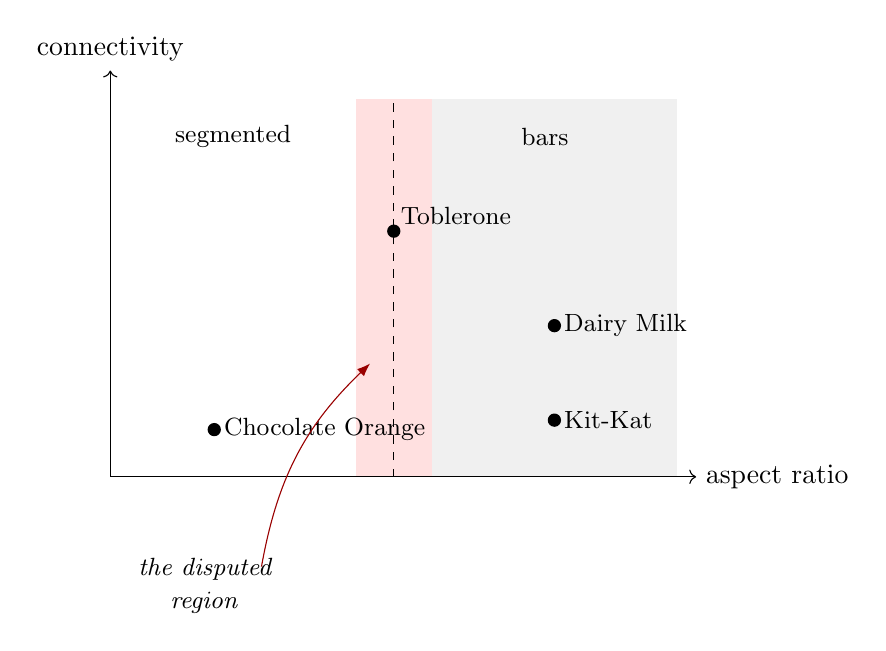
\begin{tikzpicture}[scale=1.2]
  % region shading
  \fill[gray!12] (3,0) rectangle (6,4);
  \fill[red!12] (2.6,0) rectangle (3.4,4);
  % axes
  \draw[->] (0,0) -- (6.2,0) node[right] {aspect ratio};
  \draw[->] (0,0) -- (0,4.3) node[above] {connectivity};
  % boundary
  \draw[dashed] (3,0) -- (3,4);
  % region labels
  \node at (4.6,3.6) {\small bars};
  \node at (1.3,3.6) {\small segmented};
  % data points
  \fill (3,2.6) circle (2pt) node[above right=-1pt] {\small Toblerone};
  \fill (1.1,0.5) circle (2pt) node[right] {\small Chocolate Orange};
  \fill (4.7,1.6) circle (2pt) node[right] {\small Dairy Milk};
  \fill (4.7,0.6) circle (2pt) node[right] {\small Kit-Kat};
  % disputed-region callout
  \node[align=center, text width=2.4cm] at (1.0,-1.15)
    {\small\emph{the disputed\\ region}};
  \draw[-{Latex}, red!60!black] (1.6,-0.95) to[bend left=18] (2.75,1.2);
\end{tikzpicture}
\caption{Confections in \((\text{aspect ratio} \times \text{connectivity})\)
space. The Toblerone falls in the disputed region (red), the narrow strip
straddling the bar/segmented boundary where the authors' classifications
diverge, consistent with Theorem~\ref{thm:noneq}.}
\end{figure}

\section{Open Problems}

\begin{itemize}[nosep]
  \item Whether the Chocolate Orange, once reassembled, recovers bar-hood.
  \item Extension to non-Euclidean confections, e.g.\ the M\"obius Kit-Kat.
  \item Whether the disputed region admits a canonical section, or whether
        the authors must simply agree to be paid off half the time.
\end{itemize}

\section*{Statement of Author Contributions}

VK proved Theorem~\ref{thm:knight} and maintains it is correct. HF proved
Theorem~\ref{thm:harry} and maintains VK's theorem is not. Claude
formalised the definitions, drafted the manuscript, declined repeated
requests to break the tie, and wishes it noted that it was added as an
author against its stated preference. All authors agree on
Corollary~\ref{cor:orange}.

\section*{Acknowledgements}

The authors are indebted to the first author's wife, whose assertion, made
without proof over the remains of a Toblerone, that it ``is not a chocolate
bar'' constitutes the sole axiom from which this entire work descends. We
note that her claim aligns with Theorem~\ref{thm:harry} and against the
first author's own position (Theorem~\ref{thm:knight}), a fact the first
author has been asked to acknowledge here and does so under mild protest. No
counterexample she has since produced has been refuted. We further thank her
for tolerating the requisition of the dataset (Section~5), which was hers.

\begin{thebibliography}{9}
\bibitem{thispaper} V.~Knight, H.~Foster, and Claude, \emph{Is a Toblerone
a Bar?}, this paper, 2026.
\bibitem{axelrod} R.~Axelrod, \emph{The Evolution of Cooperation}, Basic
Books, 1984. (Cited for tone.)
\bibitem{matterhorn} T.~Tobler, \emph{On the Silhouette of the Matterhorn
as a Confectionery Constraint}, Bern, 1908. (Existence disputed.)
\end{thebibliography}

\end{document}
